\part{C and Unix}\toc
\section{Introduction}
\subsection{C? UNIX? What is all this about?}
\begin{frame}{C? UNIX? What is all this about?}
  \begin{block}{Let's go for a little pool, please}
    \begin{itemize}
    \item<+-> Who never heard the word ``Unix'' \textit{before arriving} at
      Telecom Nancy?
    \item<+-> Who in the room have Linux installed on a computer at home?
    \item<+-> Who have a network of Linux boxes at home?
    \end{itemize}
  \end{block}

  \begin{block}<+->{Telecom Nancy population very heterogeneous}
    \begin{itemize}
    \item Usually about $\frac{1}{3}$ didn't heard about Unix before arriving,
      and $\frac{1}{3}$ use it already
    \item We are here to level everybody
    \item Yep, some of you already know the first lectures
      {\small(go get some maths)}
    \item But be patient, soon, everyone will be lost (including YOU!)
    \end{itemize}
  \end{block}

  \begin{block}<+->{Further Quizz}
    \begin{itemize}
    \item Could you define Unix in a word? \trou{That's an Operating System}
    \end{itemize}
  \end{block}
\end{frame}
%%%%%%%%%%%%%%%%%%%%%%%%%%%%%%%%%%%%%%%%%%%%%%%%%%%%%%%%%%%%%%%%%%%%%%%%%%%%%%
\begin{frame}{Operating System}
  \begin{block}{What is an Operating System?}
    \begin{itemize}
    \item That's the software between the applications and the hardware
    \item Handles (and protects) the resources
    \item Offers an unified interface to the applications
    \end{itemize}
  \end{block}
  \centerline{\includegraphics{fig/intro-OS-notion.fig}}
\end{frame}
%%%%%%%%%%%%%%%%%%%%%%%%%%%%%%%%%%%%%%%%%%%%%%%%%%%%%%%%%%%%%%%%%%%%%%%%%%%%%%
\begin{frame}{Operating System Basics}
  \begin{itemize}
  \item<+-> What's the Operating System on neptune host (where you do your labs)?\\
    \trou{That's Linux~~~~~~~~~~~~~~~~~~~~~~~~~~~~~~~~~~~~~~~~~~~~~~~~~~~~~~~~}
  \item<.-> What's the difference between that and the Unix we spoke about
    before?\\ 
    \trou{$Linux\in Unix$, ie Linux is one member of the greater Unix family}
  \item<.-> What other Operating System you know?\\
    \trou{Windows, Mac OS are the most popular ~~~~~~~~~~~~~~~~~~~~~~~~~~~~~~~}
  \item<.-> Any idea of the amount of existing Operating System? Guess the
    count\\
    \trou{Writing an OS is a classical practical lab, so there's really a lot
      of them}
  \item<.-> What's the link between Mac OS and the other OSes?\\
    \trou{Mac OS 9 was a specific OS family (but it's long dead); Mac OS X is a
      Unix}
  \item<.-> Why don't we speak of Windows instead?\\
    \trou{(not \textit{'cause it sucks}) Because Windows is quite too different
      from Unix}
  \item<.-> If so, why do we speak of Unix anyway?
    \begin{enumerate}
    \item \trou{It's the most widespread OS (if you include servers, embedded,
        etc ;)}
    \item \trou{Because it's heavily connected to C (Why should we study the C language?)}
    \end{enumerate}
  \end{itemize}
\end{frame}
%%%%%%%%%%%%%%%%%%%%%%%%%%%%%%%%%%%%%%%%%%%%%%%%%%%%%%%%%%%%%%%%%%%%%%%%%%%%%%
\newcounter{a}\newcounter{b}
\subsection{Why do we need to study C?}
\begin{frame}{Why should we study the C language? Huge impact}
%  \begin{block}{Because it had a huge impact on programming languages}
    \begin{itemize}
    \item C++ is an object extension of C (you cannot master C++ without C)
    \item Java is some sort of (safe) subset of C++;
    C\# is a variation of Java
    \item Several other languages have C-like syntax (Perl, Python, Ruby, PHP)
    \end{itemize}    
%  \end{block}
  \vspace{-.8\baselineskip}
  \centerline{\includegraphics[height=.7\linewidth,angle=90]{fig/intro-language-history.fig}~~%
  \rotatebox{90}{\tiny\url{http://merd.sourceforge.net/pixel/language-study/diagram.html}}~~%
  \rotatebox{90}{\tiny See also \url{http://www.digibarn.com/collections/posters/tongues/}}}
\end{frame}
%%%%%%%%%%%%%%%%%%%%%%%%%%%%%%%%%%%%%%%%%%%%%%%%%%%%%%%%%%%%%%%%%%%%%
\begin{frame}{Why should we study the C language? Widespread}
    \begin{itemize}
    \item \structure{De facto standard for System Programming:}
      Windows, OS X, Linux, BSD  in C
    \item \structure{Counting SourceForge projects.}
      Java: 18\%; C++: 17.9\%;  C: 15.9\%
    \begin{columns}
      \begin{column}{.45\linewidth}
        
        \centerline{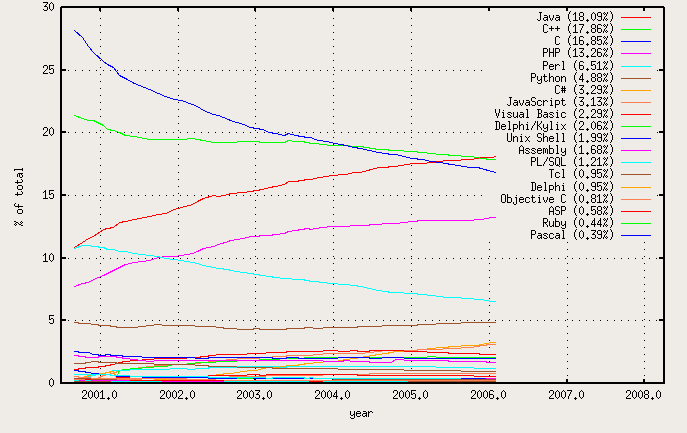
\includegraphics[width=\linewidth]{img/intro-language-sourceforge.png}%
        \rotatebox{90}{~~~\tiny\url{http://www.cs.berkeley.edu/}}
        \rotatebox{90}{~~~~~~~~\tiny\url{~flab/languages.html}}}
        
      \end{column}
    \end{columns}
\medskip
  \item \structure{Counting SLOC in Debian.}
    Quite different numbers...
    \end{itemize}

    \begin{columns}  
      \begin{column}{.35\linewidth}
        \setcounter{b}{0}
        \begin{tikzpicture}[scale=1.25]
          \foreach \p/\t/\c in {16/other/olive, 49/C/blue, 21/C++/green, 
            9/shell/yellow, 5/Java/red}
          {
            \setcounter{a}{\value{b}}
            \addtocounter{b}{\p}
            \drawSlice{\thea/100*360}{\theb/100*360}
            {\p\%}{\t}{\c}
          }        
        \end{tikzpicture}
      \end{column}
      \begin{column}{.5\linewidth}
        {\scriptsize More details:\\
        \url{http://debian-counting.libresoft.es/lenny/}\\
        See also: \url{http://www.dwheeler.com/sloc/}}

        \begin{itemize}
        \item Big codes are in C/C++ 
        \item Toy projects tend to be in Java
        \end{itemize}
        ~(but things change)
      \end{column}
    \end{columns}
\end{frame}
%%%%%%%%%%%%%%%%%%%%%%%%%%%%%%%%%%%%%%%%%%%%%%%%%%%%%%%%%%%%%%%%%%%%%
\begin{frame}{Why should we study the C language? Fast}
  \begin{itemize}
  \item \structure{C program typically execute faster than in other programs}
    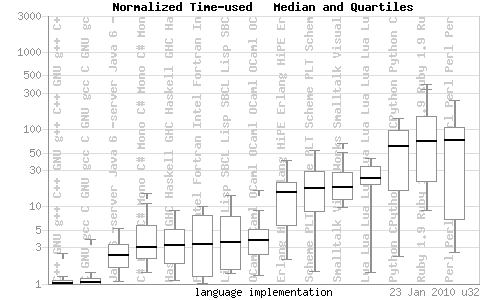
\includegraphics[width=.9\linewidth]{img/intro-shootout-fast.png}
    \rotatebox{90}{\tiny\url{http://shootout.alioth.debian.org/}}

  \item One could argue that this is because it has the best tools, but not
    only 
  \end{itemize}
\end{frame}
%%%%%%%%%%%%%%%%%%%%%%%%%%%%%%%%%%%%%%%%%%%%%%%%%%%%%%%%%%%%%%%%%%%%%
\begin{frame}{Studying the C language for educational purpose}
  \begin{block}{Understanding C helps you understanding the system as a whole}
    \begin{itemize}
    \item C is the closest high-level language to the machine
    \item Every OS are written in C, so lower interface is in C/C++ too
    \item \structure{OS/hardware co-evolution:} C conceptual model describes
      most hardware
    \end{itemize}
  \end{block}
  \begin{block}{Understanding C helps you writing better Java code}
    \begin{itemize}
    \item Java/.Net/Perl/etc hide underlying low-level mechanism
    \item But these mechanism can be very important (to performance for example)
    \item To understand how objects get passed by ref, realize that they are
      pointers
    \end{itemize}
  \end{block}
\end{frame}
%%%%%%%%%%%%%%%%%%%%%%%%%%%%%%%%%%%%%%%%%%%%%%%%%%%%%%%%%%%%%%%%%%%%%%%%%%%%%%%
\subsection{Why do we need to study C and UNIX together?}
\begin{frame}[squeeze]{Why do we need to study C and UNIX together?}
  \alert{\large Because they were invented together!}
  \vspace{-1.5\baselineskip}

    \begin{columns}
    \begin{column}{.55\linewidth}
      \includegraphics[width=\linewidth]{fig/intro-historique.fig}      
    \end{column}
    \begin{column}{.45\linewidth}
      \begin{block}{Unix history}        
        \begin{description}
        \item[1965] MULTICS: ambitious system project {\small(Bell Labs)}
        \item[1969] Bell Labs give up  \textsc{Multics}, 
          \textsc{Unics} begins 
        \item[1970] Unix: Official  Bell Labs project
        \item[1973] Rewrite in C\\
          Distribution to universities\\
          Sold by AT\&T
        \item[80-90] Unix War: {\small BSD vs. System V}\\
        \item[90-10] Normalization Effort (POSIX)
        \end{description}
      \end{block}\vspace{-\baselineskip}

      \begin{block}{C history}
        \begin{description}
        \item[1967] BCPL used at Bell Labs; 
        \item[1968] B [Thompson]: simplification
        \item[1971] C K\&R (somehow typed)
        \item[1983] C++: object oriented
        \item[1989] ANSI C; \structure{1990}: ISO C {\small(C90)}
        \item[1999] ISO C updated {\small(C99)}
        \end{description}
      \end{block}
    \end{column}
  \end{columns}
\end{frame}
%%%%%%%%%%%%%%%%%%%%%%%%%%%%%%%%%%%%%%%%%%%%%%%%%%%%%%%%%%%%%%%%%%%%%%%%%%%%%%%
\begin{frame}[squeeze]{What is Special About C?}
  \begin{block}{Low Level: sort of abstract assembly language of historical
      processors}
    \begin{itemize}
    \item Was invented on a PDP-11 with 24kb of memory: KISS!
      % The development of the C language, Dennis Ritchie.
    \item Process memory visible as an array of bytes
    \item Nothing in the language will prevent you from doing (really) stupid
      things
    \end{itemize}
    \textit{\small C combines the power of assembler with the portability of
      assembler.}

  \end{block}  
  \begin{block}{Extensible: most higher-level features doable in C}
    \begin{itemize}
    \item Self-modifying code, Introspection, Code migration, etc.
      (but all by yourself)
    \item (actually, JVM partially written in C/C++)
    \end{itemize}
    \textit{\small If you can't do it in ANSI C, it isn't worth doing.}
  \end{block}

  \begin{block}{Relatively Stable: almost backward compatible since seventies}
    \begin{itemize}
    \item Other languages got heavily lifted too often (but some heritages
      unpleasant)
    \end{itemize}
  \end{block}

  \begin{block}{C has hardly any runtime system}
    \begin{itemize}
    \item Small footprint, easily ported to new architectures 
      {\small (need to reinvent the wheel)}
    \end{itemize}
  \end{block}
\end{frame}
%%%%%%%%%%%%%%%%%%%%%%%%%%%%%%%%%%%%%%%%%%%%%%%%%%%%%%%%%%%%%%%%%%%%%%%%%%%%%%
\begin{frame}{So, should we use C once studied?}
  \begin{block}{Benefits}
    \begin{itemize}
    \item More control over the execution behaviour of programs
    \item More opportunity for performance tuning
    \item Access to low-level features of system
    \end{itemize}
  \end{block}\vspace{-.5\baselineskip}
  \begin{block}{Disadvantages}
    \begin{itemize}
    \item Need to do your own memory management
    \item Typically takes more lines of code to accomplish each task
    \item More opportunity to make mistakes
    \end{itemize}
  \end{block}\vspace{-.5\baselineskip}
  \begin{block}{Summary}
    \begin{itemize}
    \item C is a powerful programming tool for experts
    \item Presents many potential hazards for novices
    \item Helps you to understand low-level execution ideas
    \item Helps transforming you from a novice to an expert
    \item[$\leadsto$] Use it when you need it, avoid it when you don't need it
    \end{itemize}
  \end{block}  
\end{frame}
%%%%%%%%%%%%%%%%%%%%%%%%%%%%%%%%%%%%%%%%%%%%%%%%%%%%%%%%%%%%%%%%%%%%%%%%%%%%%
\section{C as Second Language}\sectionpage
\subsection{C vs. Java}
\begin{frame}{C as Second Language}
  \begin{block}{Similarities between C and Java}
    \begin{itemize}
    \item \structure{Operators}
      \begin{itemize}
      \item \structure{Arithmetic} (+,-,*,/,\% ;  ++,- -,*=,\ldots);
        \structure{Bitwise} (\&,$|$,\^{},!,$<<$,$>>$)
      \item \structure{Relational} ($<$,$>$,$<$=,$>$=,==,!=);
      \structure{Logical} \&\&, $||$, !, (a?b:c)
      \end{itemize}
    \item \structure{Keywords and Language Constructs}\vspace{-.5\baselineskip}
      \begin{columns}
        \begin{column}{.5\linewidth}
          \begin{itemize}
          \item \texttt{if( )\{ \} else \{ \}}
          \item \texttt{while( )\{ \}}
          \item \texttt{switch( ) \{ case 0: ... \}}
          \end{itemize}
        \end{column}
        \begin{column}{.45\linewidth}
          \begin{itemize}
          \item \texttt{for(i=0; i<100; i++)\{ \}}
          \item \texttt{do \{ \} while( )}
          \item \texttt{break}, \texttt{continue}, \texttt{return}
          \end{itemize}
        \end{column}
      \end{columns}\smallskip
    \item \structure{Basic (primitive) types:} void, int, short, long; float,
      double; char.\\ {\small No boolean, use int instead  (0=False; anything
        else=True)}

    \item \structure{Function declarations:} \texttt{\small int fact(int a)\{return a==0 ? 1 : a*fact(a-1);\}}
    \end{itemize}
  \end{block}\vspace{-\baselineskip}

  \begin{block}{Differences between C and Java}
    \begin{itemize}
    \item \structure{No exception:} usually rely on int error code instead 
      {\small(and usually a pain)}
    \item \structure{No class/package/interface:} code modularity different
      {\small(not compiler-enforced)}
    \item \structure{No garbage collector:} alloc and free manually needed
      memory {\small(incredible pain)}
    \end{itemize}
  \end{block}
\end{frame}
%%%%%%%%%%%%%%%%%%%%%%%%%%%%%%%%%%%%%%%%%%%%%%%%%%%%%%%%%%%%%%%%%%%%%%%%%%
\begin{frame}[squeeze]{C as Second Language}
  \begin{block}{C seems familiar when you know Java}
    \begin{itemize}
    \item Actually, that's Java which is highly inspired from C/C++
    \item Feels like a Java without any object but with full access to
      everything 
    \end{itemize}
  \end{block}

  \begin{block}{C is like Java without comfort and without any protections}
    \begin{itemize}
    \item Standard library is poor (but huge amount of extensions)
    \item Compiler is incredibly permissive (by default)
    \item It's possible to shoot yourself in the foot in Java, that's common in
      C
    \item On error, Java displays a stack trace, C spits ``segfault'' or
      ``invalid free'' errors
    \end{itemize}
  \end{block}
  
  \begin{boitequote}{Doug Gwyn}
    Unix was not designed to stop people from doing stupid things, because
    that would also stop them from doing clever things.
  \end{boitequote}
  \begin{block}{C main specificities in a Nutshell}
    \begin{itemize}
    \item Memory fully accessible through \textit{pointers}
    \item Arrays are handled as pointer to memory
    \item Declaration syntax very similar to usage syntax (to the price of
      readability)
    \end{itemize}
  \end{block}
\end{frame}
%%%%%%%%%%%%%%%%%%%%%%%%%%%%%%%%%%%%%%%%%%%%%%%%%%%%%%%%%%%%%%%%%%%%%%%%%%%%
\subsection{How to survive in C?}
\begin{frame}{How to survive in C?}
  \begin{block}{Use the tools that can help you}
    \begin{itemize}
    \item Use the \structure{compiler warning flags} \texttt{-Wall} mandatory,
      other usefull
    \item Use a \structure{proper editor} (able of colorization, auto-indent,
      compile easily)
      \begin{itemize}
      \item \structure{Good editors:} emacs \& vi (historical),
        Eclipse{\small/CDT} (my personal favorite)
      \item \structure{Bad editor:} gedit (not good for text, BAD for code)
      \end{itemize}
    \item The \structure{debugger} (\texttt{gdb}) must become your friend
      quickly
    \item \structure{valgrind} is a piece of magic (C coding without it is
      masochism)
    \end{itemize}
  \end{block}

  \begin{block}{Don't assume you're a genius (ie, don't do stupid things ---
      yet)}
    \begin{itemize}
    \item Pay attention to the modularity of your code (not compiler-enforced anyhow)
    \item Document your code (with readable comments, or doxygen for bigger
      projects) 
    \item Get some discipline (coding convention), and stick to it
      \begin{itemize}
      \item Symbol naming (my\_variable or myVariable), indentation, etc.
      \item Which one is not very important. Pick one, and stick to it
      \end{itemize}
    \item Keep it simple: it's easy to write unreadable C code
    \end{itemize}
  \end{block}
\end{frame}
%%%%%%%%%%%%%%%%%%%%%%%%%%%%%%%%%%%%%%%%%%%%%%%%%%%%%%%%%%%%%%%%%%%%%%%%%%%%%
\begin{frame}[fragile]{Bad Style Coding as a Game}
  \begin{block}{The International Obfuscated C Code Contest
      (\url{www.ioccc.org})} 
    \begin{itemize}
    \item Yearly contest of intentionally obfuscated codes 
      {\small(in C; exist for other languages)}
    \end{itemize}
  \end{block}\vspace{-.4\baselineskip}
  \begin{block}{Example: \visible<2->{Full (interactive) Maze Escape Game}
      {\normalsize (arachnid, 2004 entry)}}\vspace{-.8\baselineskip}
    \begin{columns}
      \begin{column}{.6\linewidth}
    \vbox{\begin{Verbatim}[fontsize=\tiny]
#include <ncurses.h>/*****************************************************/
            int               m[256                   ] [         256   ],a
 ,b   ;;;   ;;;   WINDOW*w;   char*l=""   "\176qxl"   "q"   "q"   "k"   "w\
xm"   "x"   "t"         "j"         "v"         "u"         "n"         ,Q[
 ]=   "Z"   "pt!ftd`"   "qdc!`eu"   "dq!$c!nnwf"/**   ***   */"t\040\t";c(
int   u ,         int         v){                     v?m   [u]         [v-
 1]   |=2,m[u][v-1] &   48?W][v-1   ] &   15]]):0:0;u?m[u   -1][v]|=1   ,m[
 u-               1][   v]&         48?               W-1   ][v         ]&
15]   ]):0:0;v<   255   ?m[   u][v+1]|=8,m[u][v+1]&   48?   W][   v+1]&15]]
):0         :0;         u <               255   ?m[   u+1         ][v   ]|=
4,m[u+1][   v]&48?W+1][v]&15]]):0:0;W][   v]&   15]   ]);}cu(char*q){   return
 *q               ?cu   (q+         1)&         1?q   [0]               ++:
q[0   ]--   :1;   }d(   int   u ,   int/**/v,   int/**/x,   int   y){   int
Y=y   -v,   X=x         -u;   int         S,s   ;Y<         0?Y   =-Y   ,s,
s=-   1:(   s=1);X<0?X=-X,S   =-1  :(S=   1);   Y<<=   1;X<<=1;   if(X>Y){
int   f=Y               -(X   >>1   );;               while(u!=         x){
f>=   0?v+=s,f-=X:0;u   +=S   ;f+=   Y;m[u][v]|=32;mvwaddch(w,v   ,u,   m[u
 ][               v]&   64?   60:         46)         ;if         (m[   u][
v]&16){c(u,v);;   ;;;   ;;;   return;}}   }else{int   f=X   -(Y>>1);;   while
 (v   !=y         ){f   >=0         ?u   +=S,               f-=         Y:0
 ;v   +=s   ;f+=X;m[u][v]|=   32;mvwaddch(w,v   ,u,m[u][v]&64?60:46);if(m[u
 ][                     v]&         16)   {c(   u,v                     );
  ;   return;;;}}}}Z(   int/**/a,   int   b){   }e(   int/**/y,int/**/  x){
int               i ;         for         (i=         a;i               <=a
+S;i++)d(y,x,i,b),d(y,x,i,b+L);for(i=b;i<=b+L;i++)d(y,x,a,i),d(y,x,a+   S,i
 );                     ;;;         ;;;         ;;;               ;;;   ;
  mvwaddch(w,x,y,64);   ;;;   ;;;   ;;;   prefresh(   w,b,a,0,0   ,L-   1,S-1
);}             main(         int               V ,   char              *C[
  ]   ){FILE*f=   fopen(V==1?"arachnid.c"/**/   :C[   1],"r");int/**/x,y,c,
                 (source code cut here)
    \end{Verbatim}
  }%$
      \end{column}
      \begin{column}{.4\linewidth}%~\medskip
        \visible<3->{
          \begin{block}{Screenshoot}\medskip
            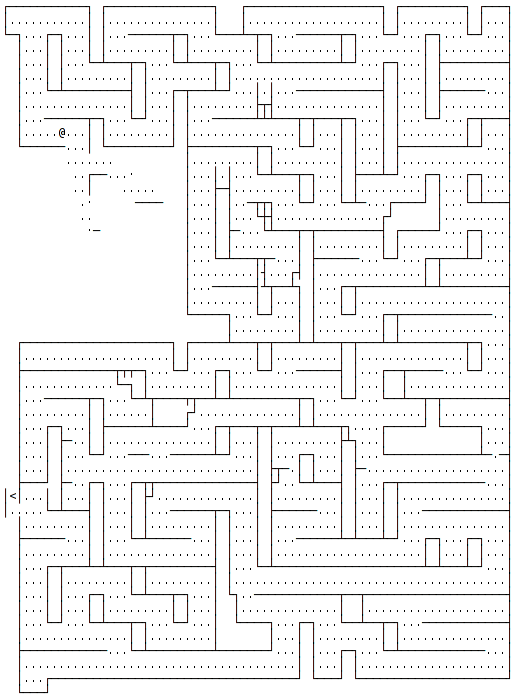
\includegraphics[width=\linewidth]{img/maze.png}          
          \end{block}
        }
      \end{column}
    \end{columns}

  \end{block}
\end{frame}
%%%%%%%%%%%%%%%%%%%%%%%%%%%%%%%%%%%%%%%%%%%%%%%%%%%%%%%%%%%%%%%%%
\begin{frame}[fragile]{Recreational Obfuscation: Phillips entry of IOCCC'88}
  \begin{Verbatim}[fontsize=\footnotesize,frame=single,label=Program code]
#include <stdio.h>
main(t,_,a)char *a;{return!0<t?t<3?main(-79,-13,a+main(-87,1-_,
main(-86,0,a+1)+a)):1,t<_?main(t+1,_,a):3,main(-94,-27+t,a)&&t==2?_<13?
main(2,_+1,"%s %d %d\n"):9:16:t<0?t<-72?main(_,t,
"@n'+,#'/*{}w+/w#cdnr/+,{}r/*de}+,/*{*+,/w{%+,/w#q#n+,/#{l,+,/n{n+,/+#n+,/#\
;#q#n+,/+k#;*+,/'r :'d*'3,}{w+K w'K:'+}e#';dq#'l \
q#'+d'K#!/+k#;q#'r}eKK#}w'r}eKK{nl]'/#;#q#n'){)#}w'){){nl]'/+#n';d}rw' i;# \
){nl]!/n{n#'; r{#w'r nc{nl]'/#{l,+'K {rw' iK{;[{nl]'/w#q#n'wk nw' \
iwk{KK{nl]!/w{%'l##w#' i; :{nl]'/*{q#'ld;r'}{nlwb!/*de}'c \
;;{nl'-{}rw]'/+,}##'*}#nc,',#nw]'/+kd'+e}+;#'rdq#w! nr'/ ') }+}{rl#'{n' ')# \
}'+}##(!!/")
:t<-50?_==*a?putchar(31[a]):main(-65,_,a+1):main((*a=='/')+t,_,a+1)
  :0<t?main(2,2,"%s"):*a=='/'||main(0,main(-61,*a,
"!ek;dc i@bK'(q)-[w]*%n+r3#l,{}:\nuwloca-O;m .vpbks,fxntdCeghiry"),a+1);}
  \end{Verbatim}    
  \begin{minipage}{.5\linewidth}
  \begin{Verbatim}[fontsize=\tiny,frame=single,label=Output]
On the first day of Christmas my true love gave to me
a partridge in a pear tree.

On the second day of Christmas my true love gave to me
two turtle doves
and a partridge in a pear tree.

On the third day of Christmas my true love gave to me
three french hens, two turtle doves
and a partridge in a pear tree.

On the fourth day of Christmas my true love gave to me
four calling birds, three french hens, two turtle doves
and a partridge in a pear tree.

On the fifth day of Christmas my true love gave to me
five gold rings;
four calling birds, three french hens, two turtle doves
and a partridge in a pear tree.

On the sixth day of Christmas my true love gave to me
six geese a-laying, five gold rings;
four calling birds, three french hens, two turtle doves
and a partridge in a pear tree.

On the seventh day of Christmas my true love gave to me
seven swans a-swimming,
six geese a-laying, five gold rings;
four calling birds, three french hens, two turtle doves
and a partridge in a pear tree.

  \end{Verbatim}    
  \end{minipage}~\begin{minipage}{.5\linewidth}
  \begin{Verbatim}[fontsize=\tiny,frame=single,label=Output (cont)]
On the eighth day of Christmas my true love gave to me
eight maids a-milking, seven swans a-swimming,
six geese a-laying, five gold rings;
four calling birds, three french hens, two turtle doves
and a partridge in a pear tree.

On the ninth day of Christmas my true love gave to me
nine ladies dancing, eight maids a-milking, seven swans a-swimming,
six geese a-laying, five gold rings;
four calling birds, three french hens, two turtle doves
and a partridge in a pear tree.

On the tenth day of Christmas my true love gave to me
ten lords a-leaping,
nine ladies dancing, eight maids a-milking, seven swans a-swimming,
six geese a-laying, five gold rings;
four calling birds, three french hens, two turtle doves
and a partridge in a pear tree.

On the eleventh day of Christmas my true love gave to me
eleven pipers piping, ten lords a-leaping,
nine ladies dancing, eight maids a-milking, seven swans a-swimming,
six geese a-laying, five gold rings;
four calling birds, three french hens, two turtle doves
and a partridge in a pear tree.

On the twelfth day of Christmas my true love gave to me
twelve drummers drumming, eleven pipers piping, ten lords a-leaping,
nine ladies dancing, eight maids a-milking, seven swans a-swimming,
six geese a-laying, five gold rings;
four calling birds, three french hens, two turtle doves
and a partridge in a pear tree.
  \end{Verbatim}
\end{minipage}
\end{frame}
%%%%%%%%%%%%%%%%%%%%%%%%%%%%%%%%%%%%%%%%%%%%%%%%%%%%%%%%%%%%%%%%%%%%%%%
%%
%% Pas possible de faire apparaitre des Verbatim en animation
%%   => dupplication du source (irk!)
%%
\begin{frame}<handout:0>[fragile,t]{Bad Style Coding as an Art}
  \begin{block}{Another example\visible<2->{: Computing Integer Square Roots}}
    \medskip
    \begin{columns}
      \begin{column}{.3\linewidth}        
    \begin{Verbatim}[fontsize=\scriptsize]
#include <stdio.h>
int l;int main(int o,char **O,
int I){char c,*D=O[1];if(o>0){
for(l=0;D[l              ];D[l
++]-=10){D   [l++]-=120;D[l]-=
110;while   (!main(0,O,l))D[l]
+=   20;   putchar((D[l]+1032)
/20   )   ;}putchar(10);}else{
c=o+     (D[I]+82)%10-(I>l/2)*
(D[I-l+I]+72)/10-9;D[I]+=I<0?0
:!(o=main(c/10,O,I-1))*((c+999
)%10-(D[I]+92)%10);}return o;}     
    \end{Verbatim}
      \end{column}
      \begin{column}{.32\linewidth}        
        \visible<2->{\structure{It actually works}\\
        \fbox{\vbox{\scriptsize\texttt{\noindent
\$ ./cheong 1234\\
35}}}\\
{\scriptsize($35\times 35=1225$; $35\times 36=1296$)}\\
\medskip\fbox{\vbox{\scriptsize\texttt{\noindent
\$ ./cheong 112233445566\\
335012}}}\\
{\scriptsize$335012\times 335012=112233040144$
$335013\times 335013=112233710169$
}}
      \end{column}
      \begin{column}{.25\linewidth}
      \end{column}
    \end{columns}
  \end{block}

\end{frame}
\begin{frame}[fragile,t]{Bad Style Coding as an Art}
  \begin{block}{Another example: Computing Interger Square Roots}
    \medskip
    \begin{columns}
      \begin{column}{.3\linewidth}        
    \begin{Verbatim}[fontsize=\scriptsize]
#include <stdio.h>
int l;int main(int o,char **O,
int I){char c,*D=O[1];if(o>0){
for(l=0;D[l              ];D[l
++]-=10){D   [l++]-=120;D[l]-=
110;while   (!main(0,O,l))D[l]
+=   20;   putchar((D[l]+1032)
/20   )   ;}putchar(10);}else{
c=o+     (D[I]+82)%10-(I>l/2)*
(D[I-l+I]+72)/10-9;D[I]+=I<0?0
:!(o=main(c/10,O,I-1))*((c+999
)%10-(D[I]+92)%10);}return o;}     
    \end{Verbatim}
      \end{column}
      \begin{column}{.32\linewidth}        
        \structure{It actually works}\\
        \fbox{\vbox{\scriptsize\texttt{\noindent
\$ ./cheong 1234\\
35}}}\\
{\scriptsize($35\times 35=1225$; $35\times 36=1296$)}\\
\medskip\fbox{\vbox{\scriptsize\texttt{\noindent
\$ ./cheong 112233445566\\
335012}}}\\
{\scriptsize$335012\times 335012=112233040144$
$335013\times 335013=112233710169$
}
      \end{column}
      \begin{column}{.25\linewidth}
        \structure{Author claim: code self-documented$\ldots$}

        \begin{Verbatim}[fontsize=\tiny]
#include <stdio.h>
int l;int main(int o,char **O,
int I){char c,*D=O[1];if(o>0){
for(l=0;D[l              ];D[l
++]-=10){D   [l++]-=120;D[l]-=
110;while   (!main(0,O,l))D[l]
+=   20;   putchar((D[l]+1032)
/20   )   ;}putchar(10);}else{
c=o+     (D[I]+82)%10-(I>l/2)*
(D[I-l+I]+72)/10-9;D[I]+=I<0?0
:!(o=main(c/10,O,I-1))*((c+999
)%10-(D[I]+92)%10);}return o;}               
        \end{Verbatim}
      \end{column}
    \end{columns}
  \end{block}

  \visible<2->{
  \begin{boitequote}{William Strunk, Jr. (1918)}
    It is an old observation that the best writers sometimes disregard the
    rules of rhetoric.  When they do so, however, the reader will usually find
    in the sentence some compensating merit, attained at the cost of the
    violation. \textbf{Unless he is certain of doing as well, he will probably
      do best to follow the rules}.
  \end{boitequote}}
\end{frame}
%%%%%%%%%%%%%%%%%%%%%%%%%%%%%%%%%%%%%%%%%%%%%%%%%%%%%%%%%%%%%%%%%%%%%%%%%%%%
\begin{frameTODO}{Bad Style Coding for Efficiency}
  Parler ici du duff device. Mais ils sont encore un peu frais pour parler
  d'horreurs pareilles. Ca leur fera meme pas peur je pense.
http://en.wikipedia.org/wiki/Duff%27s_device
\end{frameTODO}
%%%%%%%%%%%%%%%%%%%%%%%%%%%%%%%%%%%%%%%%%%%%%%%%%%%%%%%%%%%%%%%%%%%%%%%%%%%%
\begin{frame}[t]{Last one, just for fun: dhyang IOCCC'00}

  \vspace{-.5\baselineskip} Saitou Hajime image \visible<2->{that prints a
    prog} \visible<3->{that prints a prog} \visible<4->{that prints a prog}
  \visible<5->{\ldots}

  \visible<5->{Repeating endlessly "aku soku zan", Hajime's motto meaning
    \textit{slay evil imediatly}.}\medskip

  \begin{columns}
    \begin{column}{.25\linewidth}\vspace{-\baselineskip}
      \begin{block}{Source code}\medskip
        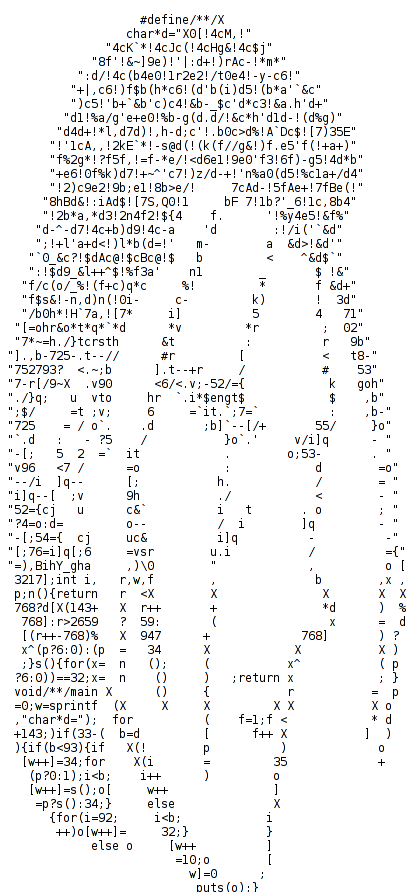
\includegraphics[width=\linewidth]{img/dhyang1.png}        
      \end{block}
    \end{column}

    \begin{column}{.3\linewidth}\vspace{-\baselineskip}
      \begin{block}<2->{Output 1}\medskip
        
\includegraphics[width=\linewidth]{img/dhyang2.png}        
      \end{block}
      \begin{block}<4->{Output 3}\medskip
        
\includegraphics[width=\linewidth]{img/dhyang4.png}        
      \end{block}
    \end{column}

    \begin{column}{.3\linewidth}\vspace{-\baselineskip}
      \begin{block}<3->{Output 2}\medskip
        
\includegraphics[width=\linewidth]{img/dhyang3.png}        
      \end{block}
      \begin{block}<5->{Output 4 (=1)}\medskip
        
\includegraphics[width=\linewidth]{img/dhyang2.png}        
      \end{block}
    \end{column}      
  \end{columns}
\end{frame}
%%%%%%%%%%%%%%%%%%%%%%%%%%%%%%%%%%%%%%%%%%%%%%%%%%%%%%%%%%%%%%%%%%%%%%%%%%%
\subsection{Your first C program}
\begin{frame}[fragile]{Your first C program}

  \begin{columns}
    \begin{column}{.47\linewidth}
      \begin{block}{The classical Hello World}\medskip
       \begin{Verbatim}[gobble=9,frame=single,fontsize=\small,label=hello.c,numbers=left]
         #include <stdio.h>
         int main(int argc, char *argv[]){
           printf("Hello, world\n");
         }
       \end{Verbatim}
      \end{block}  

      \begin{block}{Compile and run it}
        \begin{Verbatim}[gobble=9,fontsize=\small,frame=single,numbers=left]
          $ gcc -Wall hello.c -o hello
          $ ./hello
        \end{Verbatim}
      \end{block}
    \end{column}

    \begin{column}{.53\linewidth}
      \begin{block}{For the record: same in Java}\medskip
       \begin{Verbatim}[gobble=9,fontsize=\small,frame=single,label=hello.c]
         class HelloWorld {
          public static void main(String[]arg){
           System.out.println("Hello, world");
         }}
       \end{Verbatim}        
      \end{block}
      \begin{block}{Compiling and running Java code}
        \begin{Verbatim}[gobble=9,fontsize=\small,frame=single]
          $ javac HelloWorld.java
          $ java -cp . HelloWorld
        \end{Verbatim}
      \end{block}
    \end{column}
  \end{columns}
  \begin{block}{Explanations}
    \begin{itemize}
    \item \texttt{\#include} can be seen as the equivalent of \texttt{import}
      directives
    \item \texttt{main} is the \textit{entry point} of every program (same in C
      and Java)
    \end{itemize}
  \end{block}
\end{frame}
%%%%%%%%%%%%%%%%%%%%%%%%%%%%%%%%%%%%%%%%%%%%%%%%%%%%%%%%%%%%%%%%%%%%%%%%%%%%%%
\begin{frame}{C Compilation Process}
  \begin{block}{Compiling a C program involves 3 separate tools}
    \begin{enumerate}
    \item \structure{Pre-processor:} Rewrites the code according to the defined
      \textit{\alert{macros}}
      \begin{itemize}
      \item Lines begining with "\#" are macros
      \item \texttt{\#define name value}: declare a sort of automatic
        search/replace
      \item \texttt{\#define name(params) value}: search/replace but with
        arguments
      \item \texttt{\#include "file"}: inline the content of the given file
      \item \texttt{\#ifdef name}/\texttt{\#else}/\texttt{\#endif}: mask parts
        of the file if \texttt{name} is defined
      \end{itemize}
    \item \structure{Compiler:} Translates the code into assembly
    \item \structure{Linker:} Take elements in assembly and resolve library
      dependencies
      \begin{itemize}
      \item If your code uses function \texttt{cos()}, you need the math lib
      \item The linker solves a puzzle to ensure that every used function get
        defined 
      \end{itemize}
    \end{enumerate}
  \end{block}

  \begin{block}{This process is rather transparent to the user}
    \begin{itemize}
    \item You edit your code (in emacs/vi/eclipse)
    \item You launch gcc, which lauches mandatory tools automatically
    \item You mainly need to know that when you get error messages
    \end{itemize}
  \end{block}
\end{frame}
%%%%%%%%%%%%%%%%%%%%%%%%%%%%%%%%%%%%%%%%%%%%%%%%%%%%%%%%%%%%%%%%%%%%%%%%%%%%
\begin{frame}[squeeze]{What if you get error messages when compiling}
  \vspace{-.3\baselineskip}
  \begin{block}{Some examples}
    \begin{itemize}\vspace{-.3\baselineskip}
    \item \texttt{\small foo.c:71:2: error: invalid preprocessing directive
        \#deifne}\\
      \structure{The preprocessor is not happy: check file \texttt{foo.c}, line
        71, column 2}
      
    \item \texttt{\small foo.c:72: error: expected ')' before `char'}\\
      \structure{Compiler's not happy (syntax error)}
    \item \texttt{\small foo.c:74: error: redefinition of 'myFunc'\\
        foo.c:72: error: previous definition of 'myFunc' was here}\\
      \structure{Defining the same function twice makes the linker unhappy}
    \item \texttt{/usr/lib/crt1.o: In function `\_start':\\
        (.text+0x18): undefined reference to `main'\\
        collect2: ld returned 1 exit status}\\
      \structure{A function is used, but never defined} \\
      {\small(see RS lecture next year to understand the detail of the message)}
    \item \texttt{Segmentation fault ./myProg}\\
      \structure{Your program messed up the memory (valgrind knows where)}
    \end{itemize}
  \end{block}\vspace{-.8\baselineskip}

  \begin{block}{How to react when you get error messages (and you will)}
    \begin{itemize}\vspace{-.3\baselineskip}
    \item \alert{Don't panic}, even if the message seem cryptic (they often are)
    \item \alert{Read the message:} they are sometimes even understandable
    \item \alert{Don't even read the \textbf{second} message:} the parser often
      gets lost after first error
    \end{itemize}
  \end{block}
\end{frame}
%%%%%%%%%%%%%%%%%%%%%%%%%%%%%%%%%%%%%%%%%%%%%%%%%%%%%%%%%%%%%%%%%%%%%%%%%%%%%%
\begin{frame}{Conclusion on C (for now)}
  \begin{block}{C is the modern assembly language}
    \begin{itemize}
    \item It's quite prehistorical
      \begin{itemize}
      \item Compilation process not trivial (even with only one file)
      \item Cryptic error messages
      \item No fancy stuff in standard library
      \end{itemize}
    \item Programs can be really fast
      \begin{itemize}
      \item If you do them right; easy to code slow C programs too
      \end{itemize}
    \item You have the full power of doing everything
      \begin{itemize}
      \item No matter what you want to code, it's possible in C
      \item A lot of code were already developed in C (check \url{koders.com})
      \item C poses no rule to limit your imagination\ldots
      \item \ldots but there is no barrier to prevent you doing stupid things
      \end{itemize}
    \end{itemize}
  \end{block}
  \begin{block}{You need to master C to understand your machine}
    \begin{itemize}
    \item The operating system is in C, just like the virtual machines
    \item And then, you're free to use it or not\\
      Depending on whether you're seeking for fast programs or fast coding
    \end{itemize}
  \end{block}
\end{frame}
%%%%%%%%%%%%%%%%%%%%%%%%%%%%%%%%%%%%%%%%%%%%%%%%%%%%%%%%%%%%%%%%%%%%%%%%%%%%%
\section{First steps in Unix}\sectionpage
\begin{frame}[squeeze]{First steps in Unix}
  \begin{block}{This OS gives a central role to \textbf{files}}
    \begin{itemize}
    \item Contains data and executable programs (quite usual)
      \medskip
    \item \structure{Communication with user} : config files,
      \texttt{stdin}, \texttt{stdout}
    \item \structure{Communication between processes}: sockets, pipes, etc.
      \medskip
    \item \structure{Interface to the kernel}: \texttt{/proc}
    \item \structure{Interface to the hardware}: peripheral in \texttt{/dev}
    \end{itemize}
  \end{block}

  \begin{block}<2->{The \textbf{Terminal} is an interface of choice}
    \begin{itemize}
    \item Graphical interfaces exist too, but I still prefer the terminal
    \item Lots of tricks make you more efficient with the terminal\\
      (more button on my keyboard than on my mouse)
    \item If you can't do it in one step, type a one-line script directly
    \end{itemize}
  \end{block}

  \begin{block}<3->{Read The Fine Manual (RTFM)}
    \begin{itemize}
    \item The command \texttt{man} gives you access to a large corpus of
      knowledge
    \item \texttt{man prog} or \texttt{man function} $\leadsto$
      documentation of that program or function
    \end{itemize}
  \end{block}
\end{frame}
%%%%%%%%%%%%%%%%%%%%%%%%%%%%%%%%%%%%%%%%%%%%%%%%%%%%%%%%%%%%%%%%%%%%%%%%%% 
\subsection{Désignation des fichiers}
\begin{frame}<trans:0>\frametitle{Désignation des fichiers}


  \begin{block}{Désignation symbolique (nommage): \alert{Organisation
        hiérarchique}}
    
    \begin{itemize}
    \item \structure{Noeuds intermédiaires:} répertoires
      (\textit{directory} -- ce sont aussi des fichiers)
    \item \structure{Noeuds terminaux:} fichiers simples
    \item \structure{Nom absolu d'un fichier:} le chemin d'accès depuis la
      racine

    \end{itemize}
  \end{block}

  \begin{columns}
    \begin{column}{.45\textwidth}
      \begin{block}{Exemples de chemins absolus :}
        \texttt{\footnotesize
          \begin{itemize}
          \item[] /
          \item[] /bin
          \item[] /usr/local/bin/prog
          \item[] /home/bob/conf/main.tex
          \item[] /home/jim/code/main.c
          \end{itemize}      
        }  
      \end{block}     
    \end{column}

    \begin{column}{.45\textwidth}
      \includegraphics{fig/io-sgf.fig}
    \end{column}
  \end{columns}
\end{frame}

%%%%%%%%%%%%%%%%%%%%%%%%%%%%%%%%%%%%%%%%%%%%%%%%%%%%%%%%%%%%%%%%%%%%%%%%%% 

\begin{frame}<trans:0>\frametitle{Raccourcis pour simplifier la
    désignation}

  \begin{block}{Noms relatifs au répertoire courant}
    \begin{itemize}
    \item Depuis \texttt{/home/bob},~~ \texttt{conf/main.tex} =
      \texttt{/home/bob/conf/main.tex}
    \end{itemize}
  \end{block}

  \begin{block}{Abréviations}
    \begin{itemize}
    \item \structure{Répertoire père}: depuis \texttt{/home/bob},
      \texttt{\texttt{\alert{..}}/jim/code} = \texttt{/home/jim/code}
    \item \structure{Répertoire courant}: depuis \texttt{/bin},
      \texttt{\texttt{\alert{.}}/prog1} = \texttt{/bin/prog1}
    \item Depuis n'importe où, \texttt{\alert{$\sim$}}bob/ = /home/bob/ et \alert{$\sim$}/ = /home/$<$moi$>$/
    \end{itemize} 
  \end{block}

  \begin{columns}
    \begin{column}{.68\textwidth}
      \begin{block}{Liens symboliques}
        Depuis \texttt{/home/jim}
        \begin{itemize}
        \item Création du lien: \texttt{ln -s} \textit{cible nom\_du\_lien}\\
          Exemple: \texttt{ln -s /bin/prog1 monprog}
        \item \texttt{/home/jim/prog1} désigne \texttt{/bin/prog1}
        \item Si la cible est supprimée, le lien devient invalide
        \end{itemize}
      \end{block}
    \end{column}    
    \begin{column}{.3\textwidth}
      \includegraphics{fig/io-lien.fig}
    \end{column}
  \end{columns}
\end{frame}
%%%%%%%%%%%%%%%%%%%%%%%%%%%%%%%%%%%%%%%%%%%%%%%%%%%%%%%%%%%%%%%%%%%%%%%%%% 
\begin{frame}\frametitle{Règles de recherche des exécutables}
    \begin{itemize}
    \item Taper le chemin complet des exécutable (/usr/bin/ls) est lourd
    \item $\Rightarrow$ on tape le nom sans le chemin et le shell cherche
    \item Variable environnement PATH: liste de répertoires à examiner
      successivement\\
      {\footnotesize \url{/usr/local/bin:/usr/local/sbin:/sbin:/usr/sbin:/bin:/usr/bin:/usr/bin/X11}}

    \item Commande \texttt{which} indique quelle version est utilisée
    \end{itemize}

    \begin{exo}{Comment exécuter un script nommé \texttt{gcc} dans le répertoire
        courant?}
      \begin{itemize}
      \item \structure{Solution 1}: \reponse{export PATH=".:\$PATH"; gcc $<$bla$>$}
      \item \structure{Solution 2}: \reponse{./gcc $<$bla$>$}
      \end{itemize}
    \end{exo}
\end{frame}
%%%%%%%%%%%%%%%%%%%%%%%%%%%%%%%%%%%%%%%%%%%%%%%%%%%%%%%%%%%%%%%%%%%%%%%%%% 
\begin{frame}<trans:0>\frametitle{Utilisations courantes des fichiers}

  \begin{itemize}
  \item Unix: fichiers = suite d'octets sans structure interprétée par
    utilisateur
  \item Windows: différencie fichiers textes (où $\backslash$n est modifié)
    des fichiers binaires
  \end{itemize}

  \begin{block}{Programmes exécutables}
    \begin{itemize}
    \item Commandes du système ou programmes créés par un utilisateur
    \item \structure{Exemple}: \texttt{gcc -o test test.c ; ./test} \\
      \trou{Produit programme exécutable dans fichier \texttt{test}; exécute
      le programme test}
    \item \structure{Question}: pourquoi
      \underline{\textbf{./}}\texttt{test} ?
      \reponse{(car test est un binaire classique: \texttt{\tiny if test \$n -le 0;})}
    \end{itemize}
  \end{block}\vspace{-\baselineskip}

  \begin{block}{Fichiers de données}
    \begin{itemize}
    \item Documents, images, programmes sources, etc.
    \item \structure{Convention:} \trou{le suffixe indique la nature du contenu}\\
      \structure{Exemples} : .c (programme C), .o (binaire translatable,
      cf. plus loin), .h (entête C), .gif (un format d'images), .pdf
      (Portable Document Format), \textit{etc.}\\
      \structure{Remarque:} ne pas faire une confiance aveugle à
      l'extension (\textit{cf.}~ \texttt{man file})
    \end{itemize}
  \end{block}\vspace{-\baselineskip}
  
  \begin{block}{Fichiers temporaires servant pour la communication}
    \begin{itemize}
    \item Ne pas oublier de les supprimer après usage
    \item On peut aussi utiliser des tubes (\textit{cf.} RS l'an prochain)
    \end{itemize}
  \end{block}
\end{frame}
%%%%%%%%%%%%%%%%%%%%%%%%%%%%%%%%%%%%%%%%%%%%%%%%%%%%%%%%%%%%%%%%%%%%%%%%%%%%%
\subsection{Protection des fichiers}
\begin{frame}<trans:0>\frametitle{Protection des fichiers: généralités}
  \begin{block}{Définition (générale) de la sécurité}
    \begin{itemize}
    \item \structure{confidentialité} : \trou{informations accessibles aux seuls
      usagers autorisés}\vspace{-.5\baselineskip}
    \item \structure{intégrité} : \trou{pas de modifications indésirées}
      \vspace{-.5\baselineskip}
    \item \structure{contrôle d'accès} : \trou{qui a le droit de faire
        quoi} \vspace{-.5\baselineskip}
    \item \structure{authentification} : \trou{garantie qu'un usager est
        bien celui qu'il prétend être}
    \end{itemize}
  \end{block}\vspace{-.4\baselineskip}

  \begin{block}{Comment assurer la sécurité}
    \begin{itemize}
    \item Définition d'un ensemble de règles (politiques de sécurité)
      spécifiant la sécurité d'une organisation ou d'une installation
      informatique
    \item Mise en place \alert{mécanismes de protection} pour faire
      respecter ces règles
    \end{itemize}
  \end{block}\vspace{-.4\baselineskip}

  \begin{block}{Règles d'éthique}
    \begin{itemize}
    \item Protéger ses informations confidentielles (comme les projets et
      TP notés!)
    \item Ne pas tenter de contourner les mécanismes de protection (c'est
      la loi)
    \item Règles de bon usage avant tout:

      \textit{La possibilité technique de lire un fichier ne donne pas le
        droit de le faire}
    \end{itemize}
  \end{block}
     
\end{frame}
%%%%%%%%%%%%%%%%%%%%%%%%%%%%%%%%%%%%%%%%%%%%%%%%%%%%%%%%%%%%%%%%%%%%%%%%%% 
\begin{frame}<trans:0>\frametitle{Protection des fichiers sous Unix}

\begin{block}{Sécurité des fichiers dans Unix}
    \begin{itemize}
    \item Trois types d'opérations sur les fichiers : lire (r), écrire (w),
      exécuter (x)
    \item Trois classes d'utilisateurs vis à vis d'un fichier:\\
      propriétaire du fichier ; membres de son groupe ; les autres

      \begin{center}        
        \begin{tabular}{|c|c|c|}\hline
          rwx & rwx&rwx\\\hline
          \multicolumn{1}{c}{propriétaire}&
          \multicolumn{1}{c}{groupe}&
          \multicolumn{1}{c}{autres}
        \end{tabular}
      \end{center}
      
    \item[] Granularité plus fine avec les Access Control List {\small (peu
        répandus, pas étudiés ici)}
    \item Pour les répertoires, \texttt{r} = \texttt{ls}, \texttt{w} =
      créer des éléments et \texttt{x} = \texttt{cd}.
    \item \texttt{ls -l} pour consulter les droits; \texttt{chmod} pour les
      modifier  (cf. \texttt{man chmod})
    \end{itemize}
  \end{block}

  \begin{block}{Mécanisme de délégation}
    \begin{itemize}
    \item \structure{Problème} : programme dont l'exécution nécessite des
      droits que n'ont pas les usagers potentiels (\structure{exemple}:
      gestionnaire d'impression, d'affichage)
    \item \structure{Solution} (\alert{setuid} ou \alert{setgid}): ce
      programme s'exécute toujours sous l'identité du propriétaire du
      fichier; identité utilisateur momentanément modifiée\\
      identité réelle (celle de départ) vs identité effective (celle après
      setuid)
    \end{itemize}
  \end{block}
\end{frame}
%%%%%%%%%%%%%%%%%%%%%%%%%%%%%%%%%%%%%%%%%%%%%%%%%%%%%%%%%%%%%%%%%%%%%%%%%%%%%%
\subsection{Using the terminal}
\begin{frame}{Crash course on using the terminal}
  \begin{block}{Main idea}
    \begin{itemize}
    \item Your shell is somewhere in the filesystem tree (current directory)
    \item You issue commands to interact with the system
    \end{itemize}
  \end{block}\vspace{-.6\baselineskip}

  \begin{block}{Commands Basic Syntax}
    \begin{itemize}
    \item Every command follows this syntax: \code{$<$command name$>$
        $<$arguments$>$}
    \item Arguments are space separated
    \item Flags are specific arguments begining usually with \texttt{-} (minus)
    \end{itemize}
  \end{block}\vspace{-.6\baselineskip}

  \begin{block}{Minimal set of commands to remember}\medskip
    \begin{tabular}{|l|l|l|}\hline
      \textbf{Action} & \textbf{Command} & \textbf{Memoing}\\\hline
      Examine content of current dir&ls&listing \\\hline
      Know name of current dir&pwd&Print Working Directory\\\hline
      Change current dir&cd&change directory\\\hline
      Copy a file into another&cp&copy\\
      Create a new dir&mkdir&make directory\\\hline
      Destroy a file, a dir&rm, rmdir&remove\\\hline
      Usual shorthand for files and dirs&\multicolumn{2}{|l|}{.~~~..~~~/~~~\~{}~~~*~~~\~{}user}\\\hline
    \end{tabular}
  \end{block}
\end{frame}
%%%%%%%%%%%%%%%%%%%%%%%%%%%%%%%%%%%%%%%%%%%%%%%%%%%%%%%%%%%%%%%%%%%%%%%%%%
\begin{frame}[squeeze]{Using the terminal efficiently}
  \begin{block}{Common Tricks}
    \begin{itemize}
    \item Typing everything is really to slow. You need to be lazy here.
    \item \fbox{Up}/\fbox{Down}: see commands typed previously. Edit it, and
      go!
    \item \fbox{Ctrl-A}/\fbox{Ctrl-E}: jump to begin/end of line
    \item \fbox{Tab}: auto-complete what you are currently typing
%    \item \fbox{Ctrl-D}: See the possible completions
    \end{itemize}
  \end{block}\vspace{-.5\baselineskip}

  \begin{block}{Medium Tricks}
    \begin{itemize}
    \item \fbox{Ctrl-R}: begin to search a text pattern in the command
      history
    \item \fbox{\texttt{!command}}: directly relaunch the last command
      involving that \texttt{command}
    \item \fbox{\texttt{!!}}: directly relaunch the last command
    \end{itemize}
  \end{block}\vspace{-.5\baselineskip}

  \begin{block}{Advanced Tricks}
    \begin{itemize}
    \item Master your terminal (know the base commands)
    \item Assemble commands in pipe to get more advanced ones
    \item Write one-line scripts directly in the terminal
    \item Configure your environment: Declare aliases, write scripts, etc.
    \end{itemize}
  \end{block}
\end{frame}
%%%%%%%%%%%%%%%%%%%%%%%%%%%%%%%%%%%%%%%%%%%%%%%%%%%%%%%%%%%%%%%%%%%%%%%%%%%%
\begin{frame}{Conclusion on Unix (for now)}
  \begin{block}{Unix is one of the most influent operating system}
    \begin{itemize}
    \item Around since 40 years, still there for a long time
    \item Most of the OS research inovation go in Unix first
      (open source power)
    \item Other OSes become Unixes (OS X) or get portability layers (z/OS,
      windows) 
    \end{itemize}
  \end{block}

  \begin{block}{You can use that powerful tool too}
    \begin{itemize}
    \item Not as much game as on your Wii, but fully usable and free
    \item The interface may be different of what you're used to
    \item May be less intuitive at first glance, but there's a strong
      underlying philosophy
    \item Constitute a playground of choice for CS students
    \end{itemize}
  \end{block}

  \concept{Mastering this system is the goal of that course}
\end{frame}

%%% Local Variables:
%%% coding: utf-8
